\section{Architecture}
\label{sec:architecture}

\begin{itemize}
  \item Why reactive?
    \url{http://www.reactivemanifesto.org/}
    \begin{figure}[t!]
      \centering
      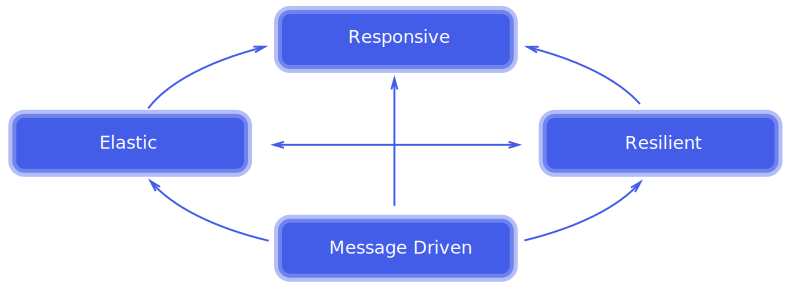
\includegraphics[width=.99\linewidth]{images/reactive-traits}
      \caption{Reactive traits.}
      \label{fig:reactive-traits}
    \end{figure}
  \item Communication by ØMQ (version 4.1.4)
  \item Docker container for clustered deployment
  \item Workers connected by routers: define worker's role and router's operating
    \begin{figure}[t!]
      \centering
      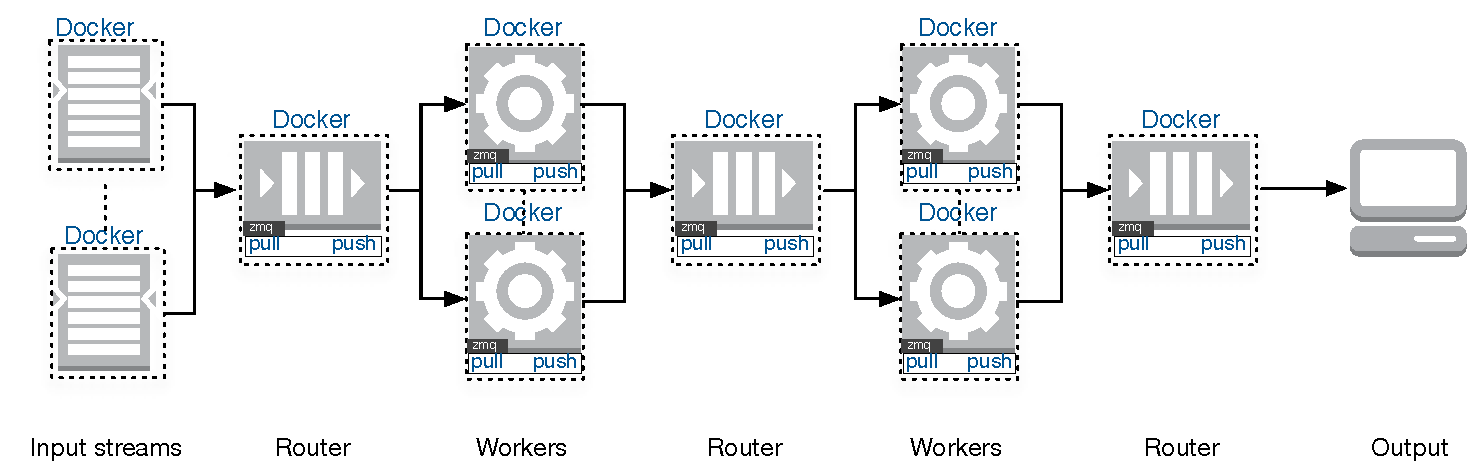
\includegraphics[width=.99\linewidth]{images/architecture_pipeline}
      \caption{Pipeline architecture.}
      \label{fig:architecture_pipeline}
    \end{figure}
  \item Fire-and-forget messaging: a messsaging pattern in which we do not expect a direct response to the message, as opposed to request-response protocols
  \item Based on Lua
\end{itemize}
